\uuid{3VHt}
\exo7id{5726}
\titre{exo7 5726}
\auteur{rouget}
\organisation{exo7}
\datecreate{2010-10-16}
\isIndication{false}
\isCorrection{true}
\chapitre{Suite et série de fonctions}
\sousChapitre{Convergence simple, uniforme, normale}

\contenu{
\texte{
Etudier les suites de fonctions suivantes (convergence simple, convergence uniforme, convergence localement uniforme)

\begin{center}
\textbf{1) (**)} $f_n(x)=\frac{nx}{1+n^2x^2}$\quad\textbf{2) (**)} $f_n(x) = e^{-x}\sum_{k=0}^{n}\frac{x^k}{k!}$\quad\textbf{3) (**)} $f_n(x) = n(1-x)^n\sin\left(\frac{\pi x}{2}\right)$. 
\end{center}
}
\reponse{
Pour tout entier naturel $n$, $f_n$ est définie sur $\Rr$ et impaire.

\textbf{Convergence simple sur $\Rr$.} Soit $x\in\Rr$.

\textbullet~Si $x =0$, pour tout entier naturel $n$, $f_n(x)= 0$ et donc $\lim_{n \rightarrow +\infty}f_n(x)=0$. 

\textbullet~Si $x\neq0$, $f_n(x)\underset{n\rightarrow+\infty}{\sim}\frac{1}{nx}$ et de nouveau $\lim_{n \rightarrow +\infty}f_n(x)=0$. 

\begin{center}
\shadowbox{
La suite de fonctions $(f_n)_{n\in\Nn}$ converge simplement sur $\Rr$ vers la fonction nulle.
}
\end{center}

\textbf{Convergence uniforme sur $\Rr$.}
On peut noter tout de suite que pour tout $n\in\Nn^*$, $f_n\left(\frac{1}{n}\right)=\frac{1}{2}$ et donc $\|f_n\|_\infty\geqslant\frac{1}{2}$. On en déduit que $\|f_n\|_\infty$ ne tend pas vers $0$ quand $n$ tend vers $+\infty$.

\begin{center}
\shadowbox{
La suite de fonctions $(f_n)_{n\in\Nn}$ ne converge pas uniformément sur $\Rr$ vers la fonction nulle.
}
\end{center}

Si on n'a pas remarqué ce qui précède, on étudie la fonction $f_n$ sur $\Rr^+$ ($f_n$ étant impaire) dans le but de déterminer $\underset{x\in\Rr}{\text{sup}}|f_n(x) - 0|$.

Soit $n\in\Nn^*$. La fonction $f_n$ est dérivable sur $\Rr^+$ et pour tout réel positif $x$, $f_n'(x) = n\frac{(1+n^2x^2)-x(n^2x)}{(1+n^2x)^2}=\frac{n(1-n^2x^2)}{(1+n^2x)^2}$. Par suite, la fonction $f_n$ est croissante sur $\left[0,\frac{1}{n}\right]$ et décroissante sur $\left[\frac{1}{n},+\infty\right[$.

Puisque la fonction $f_n$ est positive sur $\Rr^+$,  $\underset{x\in\Rr}{\text{sup}}|f_n(x) - 0|= f_n\left(\frac{1}{n}\right)=\frac{1}{2}$ qui ne tend pas vers $0$ quand $n$ tend vers l'infini.

\textbf{Convergence uniforme et localement uniforme sur $]0,+\infty[$.}
La suite de fonctions $(f_n)_{n\in\Nn}$ ne converge toujours pas uniformément vers la fonction nulle sur $]0,+\infty[$ car pour $n\geqslant1$, $\underset{x\in\Rr}{\text{sup}}|f_n(x) - 0|=\frac{1}{2}$.

 
Soit $a$ un réel strictement positif fixé. Soit $n>\frac{1}{a}$. On a $0<\frac{1}{n}<a$ et donc  la fonction $f_n$ est décroissante sur $[a,+\infty[$. Par suite, pour tout réel $x$ de $[a,+\infty[$, $0\leqslant f_n(x)\leqslant f_n(a)$.

Donc $\underset{x\in[a,+\infty[}{\text{sup}}|f_n(x) - 0|= fn(a)$ pour $n>\frac{1}{a}$. On en déduit que  $\lim_{n \rightarrow +\infty}\underset{x\in[a,+\infty[}{\text{sup}}|f_n(x) - 0|=0$.
Donc la suite de fonctions $(f_n)_{n\in\Nn}$ converge uniformément vers la fonction nulle sur tout intervalle de la forme $[a,+\infty[$ où $a > 0$ et en particulier converge localement uniformément vers la fonction nulle sur $]0,+\infty[$ mais ne converge pas uniformément vers la fonction nulle sur $]0,+\infty[$.
\textbf{Convergence simple sur $\Rr$.} Soit $x\in\Rr$. On sait que $e^x =\lim_{n \rightarrow +\infty}\sum_{k=0}^{n}\frac{x^k}{k!}$ et donc la suite $(f_n)_{n\in\Nn}$ converge simplement sur $\Rr$ vers la fonction constante $f~:~x\mapsto1$.

\textbf{Convergence uniforme sur $\Rr$ et $\Rr^+$.} $\lim_{x \rightarrow -\infty}|f_n(x)-f(x)| = +\infty$. Par suite, pour tout entier naturel $n$, la fonction $|f_n-f|$ n'est pas bornée sur $\Rr$. La suite de fonctions $(f_n)_{n\in\Nn}$ ne converge donc pas uniformément vers $f$ sur $\Rr$.

$\lim_{x \rightarrow +\infty}|f_n(x)-f(x)| = 1$ et donc $\underset{x\in[0,+\infty[}{\text{sup}}|f_n(x)-f(x)|\geqslant1$. La suite de fonctions $(f_n)_{n\in\Nn}$ ne converge donc pas uniformément vers $f$ sur $\Rr^+$.

\textbf{Convergence localement uniforme sur $\Rr$.} Soit $[a,b]$ un segment de $\Rr$.

 
Pour $n\in\Nn^*$, posons $g_n= f_n- f$. La fonction $g_n$ est dérivable sur $\Rr$ et pour $x\in\Rr$

\begin{center}
$g_n'(x)=e^{-x}\left(-\sum_{k=0}^{n}\frac{x^k}{k!}+\sum_{k=0}^{n-1}\frac{x^k}{k!}\right)=-\frac{e^{-x}x^n}{n!}$.
\end{center}

Si $n$ est pair, la fonction $g_n$ est décroissante sur $\Rr$ et s'annule en $0$.

Si $n$ est impair, la fonction $g_n$ est croissante sur $\Rr^-$, décroissante sur $\Rr^+$ et s'annule en $0$.

Dans les deux cas, si $x\in[a,b]$, $|g_n(x)|\leqslant\text{Max}\{|g_n(a)|,|g_n(b)|\}$ avec égalité effectivement obtenue pour $x=a$ ou $x=b$. Donc 

\begin{center}
$\underset{x\in[a,b]}{\text{sup}}|gn(x)|=\text{Max}\{|g_n(a)|,|g_n(b)|\}=\frac{g_n(a)+g_n(b)+|g_n(a)-g_n(b)|}{2}$.
\end{center}

Cette dernière expression tend vers $0$ quand $n$ tend vers $+\infty$. On en déduit que la suite de fonctions $(f_n)_{n\in\Nn}$ converge uniformément vers $f$ sur tout segment $[a,b]$ contenu dans $\Rr$ ou encore 

\begin{center}
\shadowbox{
la suite de fonctions $(f_n)_{n\in\Nn}$ converge localement uniformément vers la fonction $f~:~x\mapsto1$ sur $\Rr$.
}
\end{center}
Pour $x$ réel et $n$ entier naturel, on pose $f_n(x) =n(1-x)^n\sin\left(\frac{\pi}{2}x\right)$.

\textbf{Convergence simple.} Soit $x$ réel fixé. $\sin\left(\frac{\pi}{2}x\right)=0\Leftrightarrow x\in 2\Zz$. Dans ce cas, $\lim_{n \rightarrow +\infty}f_n(x) =0$.

Si $x\notin 2\Zz$, la suite $(f_n(x))_{n\in\Nn}$ converge $\Leftrightarrow$ la suite $(n(1-x)^n)_{n\in\Nn}$ converge $\Leftrightarrow |1-x| < 1 \Leftrightarrow 0 < x < 2$. Dans ce cas, $\lim_{n \rightarrow +\infty}f_n(x)=0$.

\begin{center}
\shadowbox{
La suite de fonctions $(f_n)_{n\in\Nn}$ converge simplement  vers la fonction nulle sur $[0,2]\cup 2\Zz$.
}
\end{center}

\textbf{Convergence uniforme sur $[0,2]$.} Soit  $n$ un entier naturel non nul fixé.

\begin{center}
$\underset{x\in[0,2]}{\text{sup}}|f_n(x)-0|\geqslant\left|f_n\left(\frac{1}{n}\right)\right|=n\left(1-\frac{1}{n}\right)^n\sin\left(\frac{\pi}{2n}\right)$.
\end{center}

Cette dernière expression est équivalente à $\frac{\pi}{2e}$ en $+\infty$ et en particulier ne tend pas vers $0$ quand $n$ tend vers $+\infty$. 

\begin{center}
\shadowbox{
La suite de fonctions $(f_n)_{n\in\Nn}$ ne converge pas uniformément  vers la fonction nulle sur $[0,2]$.
}
\end{center}

$$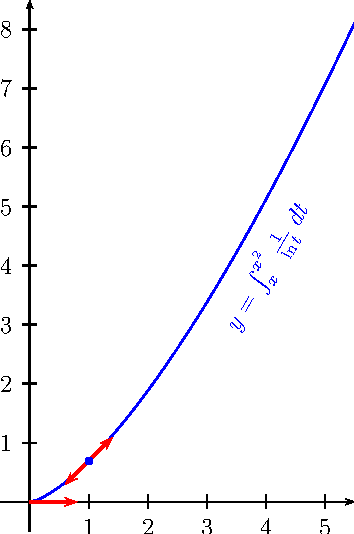
\includegraphics{../images/img005726-1}$$


\begin{center}
\shadowbox{
La suite de fonctions $(f_n)_{n\in\Nn}$ ne converge pas uniformément  vers la fonction nulle sur $[0,2]$.
}
\end{center}
}
}
